\section{Evaluation}\label{sec:evaluation}

% \review{While I found the idea behind section V very interesting, the current version
%   of this section lacks some details that would help in better understanding (1) 
%   how the approach works, and (2) the overall scope of the approach. 
%   $\\$
%   For instance, the authors state that, following [19], they try to "exercise
%   interesting patterns" by adding "admissible but redundant typing rules" like
%   G-ASTR. There are a few points that are unclear here: (1) are these rules
%   discovered manually or automatically (starting from the Redex semantics)?, (2)
%   are there any guiding principles for coming up with rules that lead to
%   interesting cases?
%   $\\$
%   Later, the authors refer to "generation rules modified to be slightly more
%   permissive" to generate "a little" ill-typed terms. Again, are these rules
%   obtained automatically or defined manually? If the latter, did you follow any
%   methodology to derive such rules? Are these rules the same as the "admissible
%   but redundant typing rules" from above?}
% \liyi{Deena? Leo? }
We evaluate~\systemname in terms of the following three aspects:
\begin{itemize}
\item\textbf{Conversion Effort:} How much developer effort is needed to annotate parts of programs to run in~\systemname?
\item\textbf{Performance Overhead:} What is the performance overhead (both runtime and memory) in using~\systemname?
\item\textbf{Security Impact:} How effective is the isolation provided by~\systemname{} in preventing security vulnerabilities?
\end{itemize}

%Our evaluation of \systemname consists of a set of tests that can be classified into Micro-benchmarks and Program Benchmarks that evaluate \systemname on WebAssembly sandbox. Consequently, all further references to sandbox refer to unchecked code in the WebAssembly Sandbox. 
%MicroBenchmarking involves evaluating performance on fundamental operations involving tainted pointers, context switching between checked and sandboxed regions, and sandboxed execution of functions.
%We further go on to evaluate \systemname on six real-world programs pertaining to diversified domains to evaluate real-world run-time and memory performance.

\subsection{Dataset}
Network-facing programs such as servers directly interact with external input, often process complex data types, and are more susceptible to security issues.
We primarily focus on network servers as they can benefit most from our partitioning approach.
We use WebAssembly (WASM) as our target sandbox. Consequently, we also want any of the selected programs to be compilable with the WASM sandbox.
We selected network servers that we could (with minimal effort) compile with the WASM compiler.
We also selected a few standalone programs suggested by the ~\checkedc team~\cite{benchmarkcc}, which are good candidates to evaluate modifications to~\checkedc.
\tbl{table:dataset} shows the program selected as part of our evaluation dataset. 


\subsection{Experimental Setup}
\label{experimentalsetup}
All experiments are performed on a 6-Core Intel i7-10700H machine with 40 GB of RAM, running Ubuntu 20.04.3 LTS.
We use WASM as our target sandbox and use a similar configuration as that of the recent work~\cite{rlbox-paper};
and Valgrind's "massif" memory profiler~\cite{seward2008valgrind} to measure the memory usage and consider the peak heap usage of an application as its memory consumption.
We measure runtime using the difference in elapsed clock cycles using~\code{clock()} API from POSIX's~\code{<time.h>} and linux's ~\code{time} command, and perform every measurement ten times and use the average as the final result.

%\myparagraph{Benchmarking Methodology}
%\systemname is evaluated in terms of performance and conversion efforts similar to that of RLBOX \cite{rlbox-paper} by recording run-time and memory overhead incurred by a \systemname in comparison to an unconverted program in generic-C/checked-C. 
%However, the scope of \systemname changes made on each of the programs is varied and the converted programs themselves are relatively tiny.
%Since each of the program is evaluated on a pre-defined test-suite that runs on a single instance of the program, sandbox creation cost is a one-time constant due to \systemname implementing RLBOX's \cite{rlbox-paper} WebAssembly sandbox API. 
%\liyi{I do not understand the following sentence, what is test-bench? }
%Run-time performance is evaluated with C's~\code{<time.h>} library by placing each of the test-bench calls within the timing scope (Program scope within which the timer runs) and measuring latency delta as a percentage. 
%\liyi{need to rewrite}
%Timing scope excludes marshaling activities within the test-case environment with an intuition that marshaling is irrelevant if tainted-ness of a pointer is propagated from the call site up until its declaration. 
%\liyi{What is Valgrind? }
%Memory overhead is measured with Valgrind's "massif" memory profiler to benchmark the peak memory usage of the Heap. Unlike the Runtime performance, Peak Memory is recorded as a relative offset to original program because most programs are extremely small in comparison to the constant overhead from the sandbox (81 KiB approx). This can further be optimized away by choosing to only compile custom Tainted wrappers for those STDLIB functions that are in use by the tainted pointers in the program. Valgrind's memory figures do not account for Sandbox's Heap allocations which are linearly proportional to sandboxed code and tainted pointers.  
%All of the evaluation was performed using 6-Core Intel i7-10700H with 40 GB of RAM, running Ubuntu 20.04.3 LTS and the benchmarks for every test were sampled as the mean of ten consecutive iterations.

\subsection{Conversion Effort}
The flexibility of~\systemname{} (\sect{subsec:otherusecases}) enables an application to be partitioned in several ways -- with varying levels of overhead and assurance. We explore the following three ways:

\noindent\emph{Checked C and Tainted Partitions ($CTP$):} This is the most comprehensive use case, where the~\cregion partition contains completely annotated Checked C code, and~\ucregion contains one or more tainted functions.
This provides the complete spatial safety of the code in~\cregion{} including isolation from~\ucregion{}.


\noindent\emph{Only Tainted Partition ($TP$):}
This is the general partitioning (\sect{subsec:otherusecases}) use case without Checked C.
This is similar to $CTP$, but~\cregion code does not use any Checked C annotations.
This provides only the isolation guarantee without spatial safety.


\noindent\emph{Only Tainted Pointers ($T_{Pr}$):}
In this use case, we only use tainted pointers, and all code lies in~\cregion.
This is needed for data isolation-only cases, where the developer might want to just isolate certain data (\eg user input) from the rest of the program.
As explained in~\sect{subsec:compilerimple}, all access through tainted pointers will be dynamically checked to ensure that every access is within sandbox.
This provides partial spatial safety by ensuring that any spatial violation involving tainted pointer cannot affect~\cregion.

{
\footnotesize
\begin{table}[]
\begin{tabular}{c|c|c|r}
\toprule
\textbf{ID} & \textbf{Program} & \textbf{Description}          & \multicolumn{1}{c}{\textbf{\begin{tabular}[c]{@{}c@{}}Size\\ (SLoc)\end{tabular}}} \\ 
\midrule
\rowcolor{black!15} 1           & ProFTPD          & High performance FTP Server   & 556 K                                                                               \\ 
2           & MicroHTTPD       & Simple HTTPD Server           & 122 K                                                                                \\ 
\rowcolor{black!15} 3           & UFTPD            & UDP based FTP Server          & 3 K                                                                               \\ 
4           & LibPNG          & Program to convert between png and pnm & 76 K                                                                               \\ 
\rowcolor{black!15}5           & TinyBigNum          & Multiple-precision integer implementation & 1.6 K                                                                               \\ 
6           & Parsons          & JSON parsing library & 3.1 K                                                                               \\ 

\bottomrule
\end{tabular}
\caption{Evaluation Dataset.}
\label{table:dataset}
\end{table}
}

%{
\scriptsize
\begin{table}[]
\begin{tabular}{c|c|c|c|r|c}
\toprule
\textbf{Program} & \textbf{\begin{tabular}[c]{@{}c@{}}Partition\\ Methodology\end{tabular}} & \textbf{\begin{tabular}[c]{@{}c@{}}Pointers\\ Annotated\end{tabular}} & \textbf{\begin{tabular}[c]{@{}c@{}}Lines in\\ \ucregion\end{tabular}} & \multicolumn{1}{c|}{\textbf{\begin{tabular}[c]{@{}c@{}}Time\\ Taken\\ (hours)\end{tabular}}} & \textbf{\begin{tabular}[c]{@{}c@{}}CVEs\\ Prevented\end{tabular}} \\ 
\midrule
\rowcolor{black!15} ProFTPD          &     $TP$                                                                     &       6                                                                &                                                                     N/A &                                                                                      1        & CVE-2010-4221                                                           \\ %\hline
png2pnm          & \multirow{2}{*}{$TP$}                                                        & \multirow{2}{*}{248}                                                     & \multirow{2}{*}{N/A}                                                    & \multirow{2}{*}{}                                                                            & \multirow{2}{*}{CVE-2018-144550}                                             \\ %\cline{1-1}
pnm2png          &                                                                          &                                                                       &                                                                      &                                                     8                                         &                                                                   \\ %\hline
\rowcolor{black!15} MicroHTTPD       &     $T_{Pr}$                                                                     &          139                                                             &                                                                     6450 &                                                                                       3       &                    N/A                                               \\ %\hline
UFTPD            &        $T_{Pr}$                                                                  &  146                                                                     &                                                                     90 &                                                           3                                   & \begin{tabular}[c]{@{}c@{}}CVE-2020-14149\\ CVE-2020-5204\end{tabular}             \\ %\hline
\rowcolor{black!15} TinyBigNum       &      $CTP$                                                                    &   69                                                                    &                                                                     30 &                                                                                        2      &                             N/A                                      \\ %\hline
Parsons          &     $CTP$                                                                     &      364                                                                 &                                                                     800 &                                                      5                                        &                                                  N/A                 \\ 
\bottomrule
\end{tabular}
\caption{Summary of our Conversion Efforts and Security Impact.}
\label{table:conversioneffort}
\end{table}
}
 
\subsubsection{Conversion Methodology}
We partitioned each program in our dataset using one of the above three methods.

Our goal is to isolate risky input processing routines from the application code.
We manually analyze each application's source code to identify which functions handle the input data and how.
We also look into previously reported vulnerabilities to identify risky input processing routines.
We picke one of the above methods to partition based on how the input data is processed.
Table ~\ref{table:conversioneffort} is a summary of our dataset partitioning.
For~\texttt{ProFTPD}, $T_{Pr}$ method is used and the input data is marked as tainted.
Consequently, five other pointers need to be marked as tainted according to the type rules. This results in a total of 6 pointer annotations. There is no code in~\ucregion as used $T_{Pr}$ method with only tainted pointers being used.
We follow the same approach for~\texttt{LibPNG} (\texttt{png2pnm} and~\texttt{pnm2png}). However, in this case, we have to annotate much more pointers (248) due to the complicated \texttt{libPNG}'s internal structures.

For~\texttt{MicroHTTPD} and~\texttt{UFTPD}, $TP$ method is used and we mark all of the direct input handled methods as tainted, which are consequently moved to the sandbox, with annotating several intermediate pointers as tainted.
For~\texttt{TinyBignum} and~\texttt{Parsons},
we follow $CTP$ and mark all input processing routines as tainted and place them in the sandbox.
The rest of the non-sandboxed code is annotated completely using~\checkedc types and placed in~\cregion.

We ensured that the partitioned programs retained their expected functionality by verifying using corresponding test suites.

\subsubsection{Conversion Effort}
The second last column shows the hour numbers for partitioning applications.
On average, it takes $\sim$ 3.5 hours for each partitioning. However, the exact time depends on the complexity of the application and the pointer usage.
Although the absolute time is high, partitioning is a one-time effort for each application.
We start by annotating functions and then iteratively fixing type-checker errors.
Most of the time (80\%) is spent on running the type-checker.
The type-checker stops at the first error without giving information about other variables that needs to be fixed. 
For an instance, in the following code:
\begin{minted}[mathescape, escapeinside=||, fontsize=\footnotesize]{c}
_TPtr<int> y = ...; 
int *z;
int *x;
|\textcolor{red}{\faRemove}| z = y;
x = z;
\end{minted}
The type-checker displays an error only for the first assignment.
However, to correctly fix it, we need to annotate both~\code{x} and~\code{y}.
If $N$ pointers need to be annotated, then in the worst case, we might have to run the type-checker $N$ times, annotating one additional pointer in every run.
We plan to fix this in our future work by making the conversion procedure automatic.
%make the type-checker display all the affected pointer variables instead of just the type errors.

\subsection{Performance Overhead}
Recent work~\cite{jangda2019not} shows that code executed as part of WASM sandbox incurs significant runtime overhead,~\ie$\sim$200\%.
To better understand our runtime overhead, we first perform micro benchmarking of additional sandbox-related operations in~\systemname{}.

\subsubsection{Micro-Benchmarking}
\Cref{fig:microbenchmarks} shows our micro-benchmarking result.
We measure the following operations as part of this:

\noindent\emph{Memory access in WASM Sandbox ($SBX_{m}$):} 
All memory accesses in a sandbox need additional verification by the sandbox runtime, which results in runtime overhead.
We perform 100K memory accesses (read and write) in a loop, measure the time inside the sandbox, and compare it with the time executed as a regular program.
%
The results (~\fig{fig:microbenchmarks}) show that we incur 156.6\% overhead for memory accesses in the WASM sandbox compared to that in a normal program.
This is inline with the observations of the recent work~\cite{jangda2019not}.

\noindent\emph{Sandbox Roundtrip ($SBX_{RT}$):}
We measure the time to make a round trip between~\cregion and sandbox (\ucregion) compared to a regular function call and return.
We create a no-op function below:
\begin{minted}[mathescape, escapeinside=||, fontsize=\footnotesize]{c}
void noop() { return; }
\end{minted}
We place this~\code{noop} function in the sandbox and measure the time to call and return from it:
\begin{minted}[mathescape, escapeinside=||, fontsize=\footnotesize]{c}
s = clock();
sandbox_noop();
e = clock();
\end{minted}
We compare the time with a regular call when \code{noop} is in~\cregion.

As shown in ~\fig{fig:microbenchmarks}, we incur an overhead of $\sim 400\%$. This is also inline with the performance reported by prior works~\cite{jangda2019not, rlbox-paper}.
This is expected because transitions to/from sandbox require context switches which are more expensive than regular function calls (\ie\code{call} and~\code{ret} instructions).

\noindent\emph{Tainted Pointer Access in~\cregion ($TP_{c}$):}
As explained in~\sect{subsec:compilerimple}, we need to perform pointer swizzling to convert the sandbox-specific representation of tainted pointers to raw addresses.
In addition, our instrumentation also checks at runtime that all tainted pointers are within the sandbox address range before accessing them.
We measure this additional overhead by comparing tainted pointer accesses with regular pointer accesses.

As shown in~\fig{fig:microbenchmarks}, we incur 34\% overhead in accessing tainted pointers in~\cregion,
 due to additional validation checks, which require executing two compare instructions for every memory access.


%\subsection{Micro-Benchmarks}
%
%
%
%\liyi{What is SBX, and how it is related to indirect-calls, pointer accesses and what is micro-benchimarks doing? Should we elaborate a little? }
%
%Figure \ref{fig:microbenchmarks} shows calls to the sandbox and sandboxed code execution to have significantly higher overhead in comparison to that of Tainted pointers. This observation suggests for sandboxing less performance intensive code and reducing the indirect calls between the two regions. Consequently, unsafe regions of code can be annotated cost-effectively by choosing to annotate the unsafe pointer references within the demarked unsafe function as tainted at the cost of losing out on the Sandbox's safety features. 
%
%\subsubsection{\textbf{Memory Access in SBX}}
%Memory access performance between the checked and the WASM region involves crafting a test case that involves a simple pointer arithmetic operation enclosed in a loop of 100k iterations. 
%
%\myparagraph{Results}
%156.6\% overhead as shown in Figure \ref{fig:microbenchmarks} is caused by the code executing in WASM Sandbox which is comparatively inefficient as WASM compiler toolchain does not support code optimization like LLVM/GCC. 
%
%
%\subsubsection{\textbf{Indirect-Calls}}
%This test involves evaluating the overhead involved in making indirect calls and is recorded by benchmarking the time taken for a sandboxed Callee (call from the checked region into the SBX) to return. This metric is evaluated against the time taken for a checked Callee (call within local scope) to return.
%
%\myparagraph{Result}
%Observed overhead is a consequence of control transfer overhead between the checked and unchecked region as mentioned in \cite{rlbox-paper}
%
%\subsubsection{\textbf{Pointer Accesses}}
%Run-time Pointer overhead is evaluated by benchmarking a test that involves 100k read/write/arithmetic operations on the pointer.
%
%\myparagraph{Result}
%34\% in overhead is the result of "Offset To Pointer" conversion and sanity checks for Taintedness inserted by \systemname at every access to the tainted pointer.   
%\myparagraph{Result:}
%Although \systemname is shown to require 50\% more time in servicing this request, this delta is made insignificant during deployment where network bandwidth relatively accounts for a bigger metric to the overall performance.

\subsubsection{Overhead on Dataset}
\label{subsec:programoverhead}
\begin{figure}
\pgfplotsset{every x tick label/.append style={font=\tiny, rotate=30}}
\pgfplotsset{every y tick label/.append style={font=\tiny}}
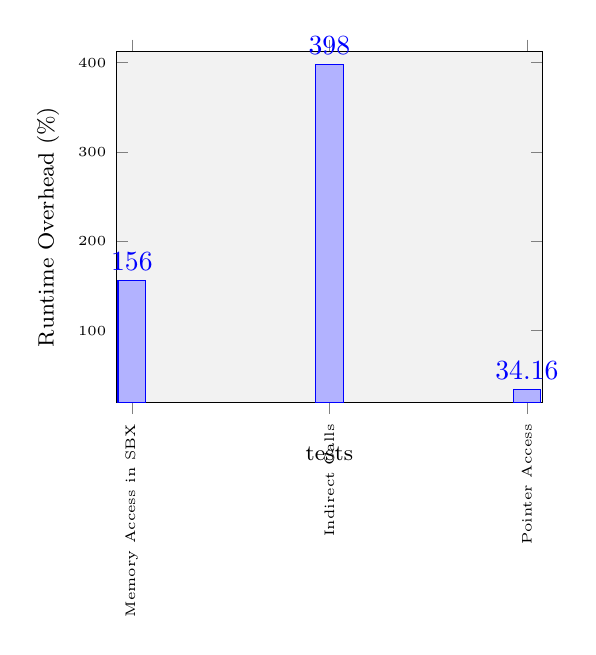
\begin{tikzpicture}  
  
\begin{axis}  
[  
    ybar,  
    enlargelimits=0.04,  
    ylabel={Runtime Overhead (\%)}, % the ylabel must precede a # symbol.  
    %xlabel={Micro-Benchmark Tests},  
    symbolic x coords={Memory Access in SBX, Indirect Calls, Pointer Access}, % these are the specification of coordinates on the x-axis.  
    xtick=data,  
    bar width=10pt,
    width=7cm,
    x tick label/.append style={font=\tiny, rotate=30},
    y tick label/.append style={font=\tiny},
    axis background/.style={fill=gray!10},
    x label style={at={(axis description cs:0.5,-0.1)},anchor=north, font=\footnotesize},
    xlabel={tests},
    ylabel style={font=\footnotesize},
     nodes near coords, % this command is used to mention the y-axis points on the top of the particular bar.  
    nodes near coords align={vertical},  
    ]  
\addplot coordinates {(Memory Access in SBX,156) (Indirect Calls, 398) (Pointer Access, 34.16)};  
  
\end{axis}  
\end{tikzpicture} 
\caption{\systemname Micro-Benchmarks.}
\label{fig:microbenchmarks}
\end{figure}

\begin{figure}
\pgfplotsset{every x tick label/.append style={font=\tiny, rotate=30}}
\pgfplotsset{every y tick label/.append style={font=\tiny}}
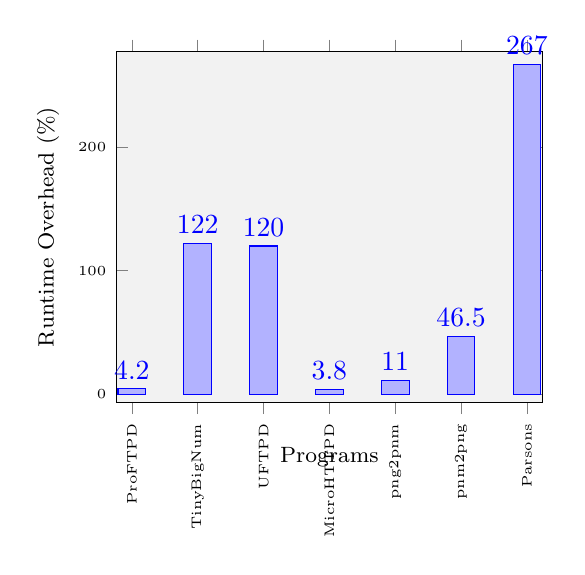
\begin{tikzpicture}  
  
\begin{axis}  
[  
    ybar,  
    enlargelimits=0.04,  
    ylabel={Runtime Overhead (\%)}, % the ylabel must precede a # symbol.  
    %xlabel={Programs},  
    symbolic x coords={ProFTPD, TinyBigNum, UFTPD, MicroHTTPD, png2pnm, pnm2png, Parsons}, % these are the specification of coordinates on the x-axis.  
    xtick=data,  
    bar width=10pt,
    width=7cm,
    x tick label/.append style={font=\tiny, rotate=30},
    y tick label/.append style={font=\tiny},
    axis background/.style={fill=gray!10},
    x label style={at={(axis description cs:0.5,-0.1)},anchor=north, font=\footnotesize},
    xlabel={Programs},
    ylabel style={font=\footnotesize},
     nodes near coords, % this command is used to mention the y-axis points on the top of the particular bar.  
    nodes near coords align={vertical},  
    ]  
\addplot coordinates {(ProFTPD,4.2) (TinyBigNum,122) (UFTPD, 120) (MicroHTTPD,3.8) (png2pnm, 11) (pnm2png, 46.5) (Parsons, 267)};  
  
\end{axis}  
\end{tikzpicture} 
\caption{Runtime Overhead of Partioned Programs.}
\label{fig:runtimeoverhead}
\end{figure}



%\begin{figure}
\pgfplotsset{every x tick label/.append style={font=\tiny, rotate=30}}
\pgfplotsset{every y tick label/.append style={font=\tiny}}
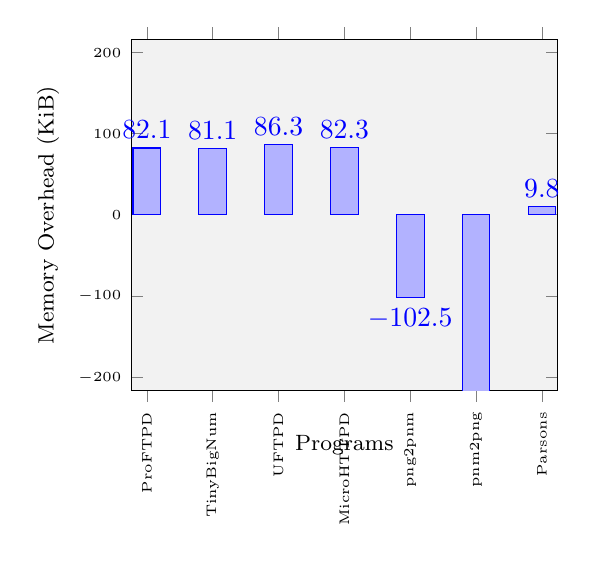
\begin{tikzpicture}  
  
\begin{axis}  
[  
    ybar,  
    ymin=-200, ymax=+200,
    enlargelimits=0.04,  
    ylabel={Memory Overhead (KiB)}, % the ylabel must precede a # symbol.  
    %xlabel={Programs},  
    symbolic x coords={ProFTPD, TinyBigNum, UFTPD, MicroHTTPD, png2pnm, pnm2png, Parsons}, % these are the specification of coordinates on the x-axis.  
    xtick=data,  
    bar width=10pt,
    width=7cm,
    x tick label/.append style={font=\tiny, rotate=30},
    y tick label/.append style={font=\tiny},
    axis background/.style={fill=gray!10},
    x label style={at={(axis description cs:0.5,-0.1)},anchor=north, font=\footnotesize},
    xlabel={Programs},
    ylabel style={font=\footnotesize},
     nodes near coords, % this command is used to mention the y-axis points on the top of the particular bar.  
    nodes near coords align={vertical},  
    ]  
\addplot coordinates {(ProFTPD,82.1) (TinyBigNum,81.1) (UFTPD, 86.3) (MicroHTTPD,82.3) (png2pnm, -102.5) (pnm2png, -51000) (Parsons, 9.8)};  
  
\end{axis}  
\end{tikzpicture} 
\caption{Memory Overhead of Partioned Programs.}
\label{fig:memoryoverhead}
\end{figure}

The first set of bars in~\Cref{fig:runtimeoverhead} shows the overhead of the partitioned programs.
%It is interesting to see a lot of variance in the runtime overhead.
The runtime overhead is proportional to the execution time 
spent in the sandbox and the number of transitions between~\cregion and the sandbox,
which coincides with the sandbox execution overhead observation in the micro-benchmarks experiments (\Cref{fig:microbenchmarks}).
\Cref{table:conversioneffort} shows the numbers of lines in the sandbox for our partitioned programs.
For~\texttt{ProFTPD}, we used only tainted pointers without code in the sandbox and transitions to/from the sandbox.
Consequently, the overhead is less than 4.2\%.
For~\texttt{UFTPD} and~\texttt{MicroHTTPD}, we sandboxed only request handlers (relatively small)
that parse messages and return the actions that need to be performed.
The server only invokes these handlers on particular requests resulting in less transitions with the sandbox.
As expected, the overhead is also less in these cases.
For~\texttt{TinyBigNum} and~\texttt{Parsons}, the overhead is high because of the relatively large amount of code in sandbox region.
In both applications, we place the frequently used parsing functions in the sandbox 
resulting in a lot of sandbox transitions with most of them in a loop.
The case is slightly different in~\texttt{pnm2png} and~\texttt{png2pnm},
where we made the entire~\code{png} structure tainted, 
which resulted in dynamic checks every time when the~\code{png} struct is accessed.
In summary, our results indicate that the runtime overhead largely depends on the sandbox.

\noindent\textbf{Overhead of only~\systemname{}.}
To verify the impact of the sandbox on the overall program runtime, we perform a NO-OP sandbox experiment.
Our goal is to measure the runtime overhead introduced ONLY by~\systemname{}.
We perform this experiment by skipping sandboxing.
Specifically, we run the completely annotated program as a regular application without any partitioning.
However, we compile the annotated program with~\systemname compiler, which will add the relevant runtime checks (\sect{subsec:compilerimple}).
We modify the instrumentation on~\code{taint}ed pointers to check for a valid pointer (instead of within sandbox bounds) -- this will add the same amount of checks as in sandboxing case, but the comparison values will be different.

Our evaluation of ~\systemname{} with NO-OP Sandbox was performed on two programs with the largest overheads in our dataset. With parsons, we see an average run-time overhead of 1.94\% as is expected as parsons (($T_{Pr}$)) gave us an overhead of only 9\%. With TinyBigNum, we see an overhead of 54.7\%, and is expected referring to the figure ~\ref{fig:microbenchmarks}, as TinyBigNum is pointer intensive with pointer operations inside nested loops.     
This shows that~\systemname{} fundamentally has the least overhead.
%The second set of bars in~\fig{fig:runtimeoverhead} shows the runtime overhead. The overhead is negligible in all cases.
%This shows that~\systemname{} fundamentally has the least overhead.
%We modify the instrumentation on~\code{tainted} pointers to check for a valid pointer (instead of within sandbox bounds) -- this will add the same amount of checks as in sandboxing case, but the comparison values will be different.
%The marked \textcolor{red}{red} set of bars in~\fig{fig:runtimeoverhead} shows the runtime overhead. The overhead is negligible in all cases.
%This shows that~\systemname{} fundamentally has the least overhead.

%The result indicates a higher overhead than the non-sandboxing cases but much less overhead than the heavy sandboxing cases.
%In summary:
%\begin{itemize}
%  \item Runtime overhead is proportional to the extent of annotated pointers, sandboxed code, and transitions between~\cregion and sandbox.
%  \item Using tainted pointers with compiler generated dynamic checks is preferred than placing code in sandbox.
%  \item Different C to \systemname conversion methods affect the overhead performance, which is our major future work.
%\end{itemize}

\subsubsection{Memory Overhead}
All programs have a constant memory overhead ($\sim$81 KB) mainly for sandbox and a few variables related to creating sandbox and other helper functions.
However, similar to the original~\checkedc,~\systemname{} itself does not add any memory overhead,
because the compilation of \code{tainted} pointers do not come with any metadata.
%This is expected because, similar to~\checkedc types, ~\code{taint}ed pointers also do not have metadata and have the same runtime representation as regular pointers.

%ProFTPD's run-time overhead is expected as our conversion was small and strictly encapsulates CVE-2010-4221.
%Since UFTPD's test-suite lacks coverage for some of the \systemname changes, we manually write a script for 3 Tests that each trigger "quote CWD", "quote PORT", and FTP "get file" on a 4.0K file, following which, we record overhead as described in ~\ref{experimentalsetup}.
%Run-time overhead for UFTPD is expected as the sandboxed code was less performance intensive and FTP-protocol by itself overshadows \systemname's overhead. 

%Our evaluation of \systemname's performance results on the dataset yields the observations:
%\begin{itemize}
%  \item Run-time Overhead is proportional to the extent of 
%annotated pointers and sandboxed code.
%  \item Marshalling can be avoided if Taintedness of a pointer is propagated across its data-flow.
%  \item Marshalling might sometimes be relatively cost-effective instead of propagating the taintedness of a pointer throughout its data-flow. 
%\end{itemize}


\subsection{Security Impact}
\label{subsec:securityimpact}
The last column of the Table ~\ref{table:conversioneffort} shows the list of all spatial safety vulnerabilities in the functions that have tainted types or are isolated in the~\ucregion{}.
We re-introduced these bugs in the annotated program and checked whether these bugs could be triggered by the corresponding crashing input or exploit (if available).
We also manually verified whether the bug can be triggered or prevented by~\systemname{}.
As expected,~\emph{all vulnerabilities} are prevented by~\systemname{}.

The symbols~\vulprevented{} and~\vulisolated{} indicate whether the vulnerability was detected by our dynamic instrumentation or isolated in the sandbox, respectively.
This shows that~\systemname{} provides an effective mechanism to prevent spatial safety vulnerabilities.

% 
%\leo{The following is extremely
%  weak. ``Most of them'', were there any that weren't? Which ones? For
%  the ones that were, mention github issues.}  The random generator,
%equipped with the conversion tool, successfully found a few minor
%errors in the clang compiler, most of them were already issues in the
%git bug reports. For example, we discovered that while the ternary
%operator is implemented in the compiler it cannot handle complex
%bounds types in the branches. The static analysis is not sophisticated
%enough to properly detect that both branches have the same type. While
%not precisely a bug, the clang compiler does not permit memory for
%null terminated arrays to be allocated with calloc. Although calloc
%fills all spaces in memory with null, the compiler does not recognize
%this and claims that it is an unsafe cast.


% Recall that our
% formal model makes liberal use of bounds annotations in literals and
% the heap. 


% In order to get a better understanding of the formalism we wrote it in
% redex. This allowed us to make sure that expressions were well-typed
% and evaluated to what we expected. It also was helpful for use in
% prototyping; new features could first be added to the redex model to
% see how they interacted with the existing language. This model was
% slightly larger than the Coq model and there are some differences in
% the type systems. We included top level functions and conditional
% expressions. All of these extra expressions are still expressible in
% the coq model, for example functions can be represented as nested let
% expressions. In the Coq model variables are stored on a stack while in
% the Redex model the variables are simply looked up in the context. In
% general the Redex model is easier to modify and slightly closer to the
% actual Checked-C specifications. Instead of using the model for a
% static proof, we used it to increase our certainty of the accuracy of
% the model.


% \item Describe the random testing generator setup and the properties
%   to test.
% \yiyun{Deena's description of the implementation details. I tried
%   integrating the ones that I find relevant/interesting to the text above. Maybe we can
%   add more if we have some space to fill in.}
% In order for our guarantee of safety to hold, we need to know that our
% model acurately reflects the CheckedC clang compiler. Safety is proved
% for the Coq model, but it is significantly smaller than the actual
% language. The Redex model is a combination of both. It is written in
% the same style as the formalism but has slightly more of Checked-C's
% extra features. If expressions from the Redex model display the same
% behavior as equivalent programs in Checked-C then we have greater
% certainty that our model is useful. We built a random testing
% generator to increase this certainty.

  % \item Describe the bug findings from the random testing against the Checked-C compiler.
%   \leo{This is now integrated above}
% The generator was helpful in finding bugs in the redex model. Several things failed to typecheck that should have been well typed, and the generator was able to catch them. The generated code also found a few minor errors in the clang compiler, most of them were already issues in the git bug reports. For example we discovered that while the ternary operator is implemented in the compiler it cannot handle complex bounds types in the branches. The static analysis is not sophisticated enough to properly detect that both branches have the same type. While not precisely a bug, the clang compiler does not permit memory for null terminated arrays to be allocated with calloc. Although calloc fills all spaces in memory with null, the compiler does not recognize this and claims that it is an unsafe cast. In the Redex model there is no issue with this. A few other minor things were brought to light in the implementation of the generator. The main use was to increase certainty that the behavior in the formal model accurately matched the clang compiler.
%  
% % \end{itemize}


% \begin{itemize}
%  
% \item Show that why the formal semantics/type-system defined for Checked-C is useful. 
% Since we have certainty that our model reflects the clang compiler the model is very useful. Proofs are easier on the smaller model, so we can show  that certain things are true for it. Since the Redex model is between the formalism and the clang version we can have certainty that properties we expect are actually true for the clang version.
%  
% \begin{itemize}
% \item Show some bug findings. 
% \item Show the properties that we can guarantee for Checked-C based on the type-system and blame theorem.
% \item Maybe other useful tools that can be extracted from the Redex model.
%  
% \end{itemize}
%  
% \end{itemize}
